% encoding: utf8
% !TEX encoding = utf8
% !TeX spellcheck = pl_PL

\chapter{Specyfikacja systemu \label{chap:specyfikacja_systemu}}
Sterowanie impedancyjne w~przestrzeni operacyjnej zastosowane w~robocie Velma kompensuje jedynie masę członów własnych. Gdy manipulator chwyci narzędzie powstaje znaczny uchyb, który nie jest kompensowany. W~przypadku chwycenia przedmiotu o~dużej masie, ramię robota jest wręcz unieruchomione. Potrzebne jest gotowe narzędzie rozwiązujące opisany problem w sprawny i szybki sposób. Trzeba zmodyfikować podsystem \textit{velma\_core\_cs} w celu implementacji algorytmu pozwalającego na skompensowanie masy chwytanego narzędzia. 

Implementacja rozwiązania z sekcji \ref{chap:rozw_model} rodzi sporo problemów. W praktyce trudne jest zbudowanie odpowiedniego zadania optymalizacji, które zagwarantuje na tyle dobry model, że grawitacja będzie odpowiednio kompensowana. Dodatkowo optymalizacja obliczana jest na tyle wolno, że nie ma możliwości umieszczenia estymatora tego modelu jako jeden z komponentów podsystemu sterowania \textit{velma\_core\_cs}. Komponent musiałby zostać umieszczony w nowym agencie, który pracuje z mniejszą niż cały system częstotliwością i komunikuje się z systemem robota za pośrednictwem interfejsu ROSa. W początkowej fazie, gdy przedmiot zostanie chwycony najczęściej ramiona robota zostają nieruchome, bo grawitacja chwyconego narzędzia nie jest kompensowana. Wtedy estymacja modelu jest wyjątkowo niedokładna. W początkowej fazie należałoby stosować uproszczony model tylko po to żeby robot podniósł przedmiot. Dopiero po kilku ruchach, gdy zadanie optymalizacji zostanie poprawnie rozwiązane, można wprowadzić właściwy model z użyciem narzędzi logiki rozmytej.

Wspomniane wady były podstawą decyzji o implementacji rozwiązania z sekcji \ref{chap:rozw_pid}. Główną wadą jest niemożność wyekstrahowania danych dotyczących narzędzia które chwyta robot. Kolejną wadą może być lekkie usztywnienie stawów. Nie powinno mieć dużego znaczenia z dwóch powodów. W sterowaniu impedancyjnym w przestrzeni operacyjnej wirtualna sprężyna jest zawieszona pomiędzy chwytakiem a punktem zadanym, a nie w konkretnych stawach robota. Do tego zakładamy niskie współczynniki członu całkującego.


\section{Wymagania}
Konkretne wymagania są podyktowane środowiskiem badawczym oraz potrzebami Zespołu Programowania Robotów i Systemów Rozpoznających. 
\begin{itemize}
	\item System dostarcza gotowe komponenty potrzebne do pracy ramienia, w~szczególności: generatora trajektorii, interpolatora oraz wyznaczania kinematyki prostej 
	\item System pozyskuje dane o~otoczeniu na podstawie odczytów z~czujników położenia stawów.
	\item System samodzielnie kompensuje siłę grawitacji związaną z~masą wszystkich członów robota.
	\item Parametry chwytanego obiektu związane z~masą i inercją nie są znane i~mogą być zmienne w~czasie.
\end{itemize}

\section{Założenia}
Algorytm kompensacji grawitacji musi wyliczać dodatkowy moment w~stawach robota. Do momentów obrotowych wyliczanych na postawie  prawa sterowania impendancyjnego w~przestrzeni operacyjnej robota należy dodać te związane z~kompensacją masy narzędzia.
\begin{itemize}
	\item Wyliczone przez prawo sterowania momenty zadawane w~stawach zostaną zmodyfikowane przez algorytm kompensacji grawitacji
	\item Algorytm kompensacji ma minimalizować uchyb statyczny wynikający z~chwycenia przedmiotu o~nieznanej masie i~inercji.
	\item  Trajektoria końcówki ramienia powinna być zbliżona do trajektorii analogicznego ruchu bez uchwyconego przedmiotu.
	\item Algorytm kompensacji nie może zaburzać cech sterowania imedancyjnego pozwalających na uginanie się robota w~momencie kolizji
\end{itemize}


\section{Przypadki użycia}
Przypadki użycia (rys. \ref{fig:usecase}) odzwierciedlają pracę systemu po modyfikacji. Algorytm kompensujący ma działać przez cały czas pracy robota gdy pracuje z~narzędziem. Przypadki użycia są zbieżne z~przypadkami użycia robota kiedy pracuje w~trybie sterowania impedancyjnego.

\begin{figure}[H]
	\centering
	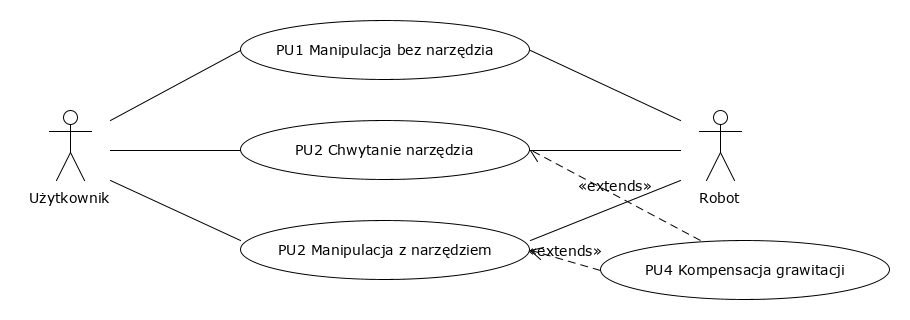
\includegraphics[width=.9\textwidth]{images/usecase.png}
	\caption{Diagram przypadków użycia robota z~uwzględnieniem algorytmu kompensacji grawitacji}
	\label{fig:usecase}
\end{figure}


Aktorami korzystającymi z~systemu są:
\begin{itemize}
	\item \textbf{Robot} - robot wykonujący zadanie chwycenia obiektu
	\item \textbf{Użytkownik} - system zewnętrzny wydający polecenia
\end{itemize}


Można wyszczególnić następujące przypadki użycia:
\begin{itemize}
	\item \textbf{PU1 Manipulacja bez narzędzia} - Konfiguracja ramienia robota może się zmieniać lecz robot nie trzyma żadnego narzędzia. Algorytm kompensacji grawitacji nie powinien zmieniać prawa sterowania. 
	\item \textbf{PU2 Chwytanie narzędzia} - Robot zaciska chwytak na narzędziu o~nieznanych parametrach a~następnie je podnosi.  
	\item \textbf{PU3 Manipulacja z~narzędziem} - Konfiguracja ramienia może się zmieniać a algorytm kompensacji grawitacji powinien przeciwdziałać sile grawitacji chwyconego narzędzia.
	\item \textbf{PU4 Kompensacja grawitacji} - Robot kompensuje siłę grawitacji chwyconego narzędzia
\end{itemize}



